\chapter{Prodotto finale}
\label{cap:prodotto finale}

\section{Pagina iniziale}
Una volta effettuato il \textit{login} l'utente può scegliere il modulo a cui vuole accedere della webapp. L'utente, accedendo al modulo Ticket, si troverà in una pagina che è composta da due sezioni:
\begin{itemize}
\item \textbf{Home Ticet};
\item \textbf{Menu Ticket}.
\end{itemize}

\subsection{Home Ticket}
La prima pagina visualizzata è la pagina di \textbf{Home Ticket}. In questa pagina sono presenti tre liste, ognuna con una modalità di visualizzazione di ticket diversa:
\begin{itemize}
\item \textbf{Aperti da me}: visualizza tutti i ticket aperti dall'utente che sta visualizzando la pagina;
\item \textbf{Assegnati a me}: visualizza tutti i ticket assegnati all'utente che sta visualizzando la pagina. Infatti un dipendente CWBI visualizzerà i ticket assegnati a lui.
\item \textbf{Recenti}: visualizza gli ultimi dieci ticket aperti, in generale.
\end{itemize}

\begin{figure}[H]
	\centering
    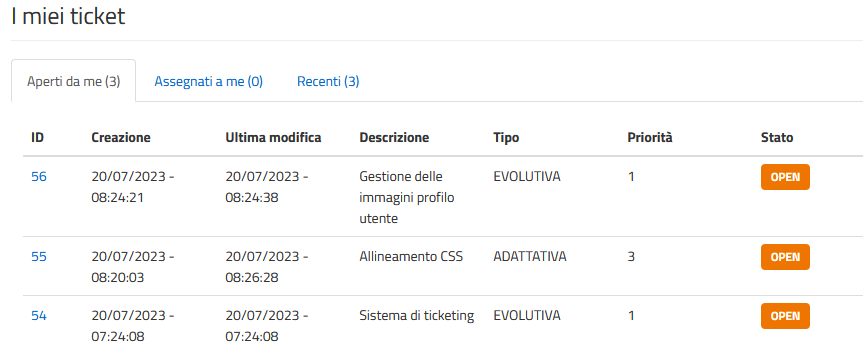
\includegraphics[width=1.1\columnwidth]{ticketApertidaMe1} 
    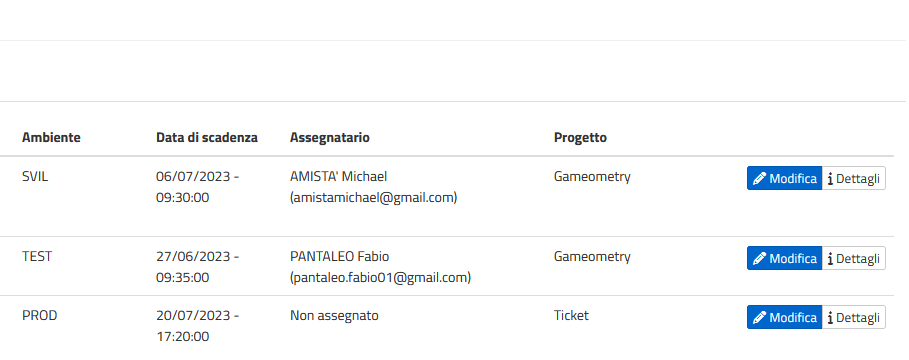
\includegraphics[width=1.1\columnwidth]{ticketApertidaMe2} 
    \caption{Home Ticket}
\end{figure}

\subsection{Menu Ticket}
La seconda sezione disponibile all'entrata nel modulo Ticket è la pagina che mostra il menù, in cui si potrà scegliere di aprire un nuovo ticket oppure effettuare una ricerca.
 
\begin{figure}[H]
	\centering
    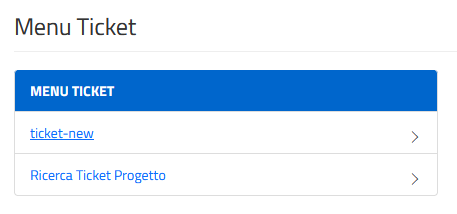
\includegraphics[width=0.7\columnwidth]{menu} 
    \caption{Menu Ticket}
\end{figure}

\newpage

\section{Nuovo Ticket}
La creazione di un nuovo ticket si divide in due step:
\begin{enumerate}
\item Si deve scegliere l'azienda che sta aprendo il nuovo ticket;
\item In base all'azienda scelta, vengono visualizzati i progetti disponibili su cui aprire il ticket; si compilano gli altri campi per l'apertura.
\end{enumerate}

 
\begin{figure}[H]
\bigskip
	\centering
    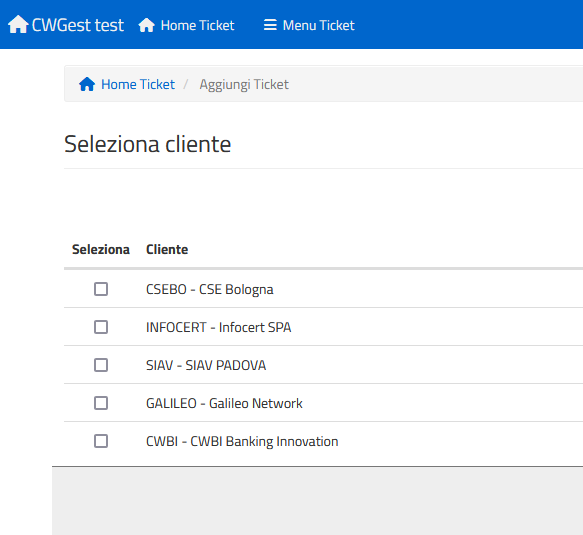
\includegraphics[width=0.7\columnwidth]{NewTicket-Step1} 
    \caption{Nuovo Ticket - Step 1}
\end{figure}

\begin{figure}[H]
\bigskip
	\centering
	
    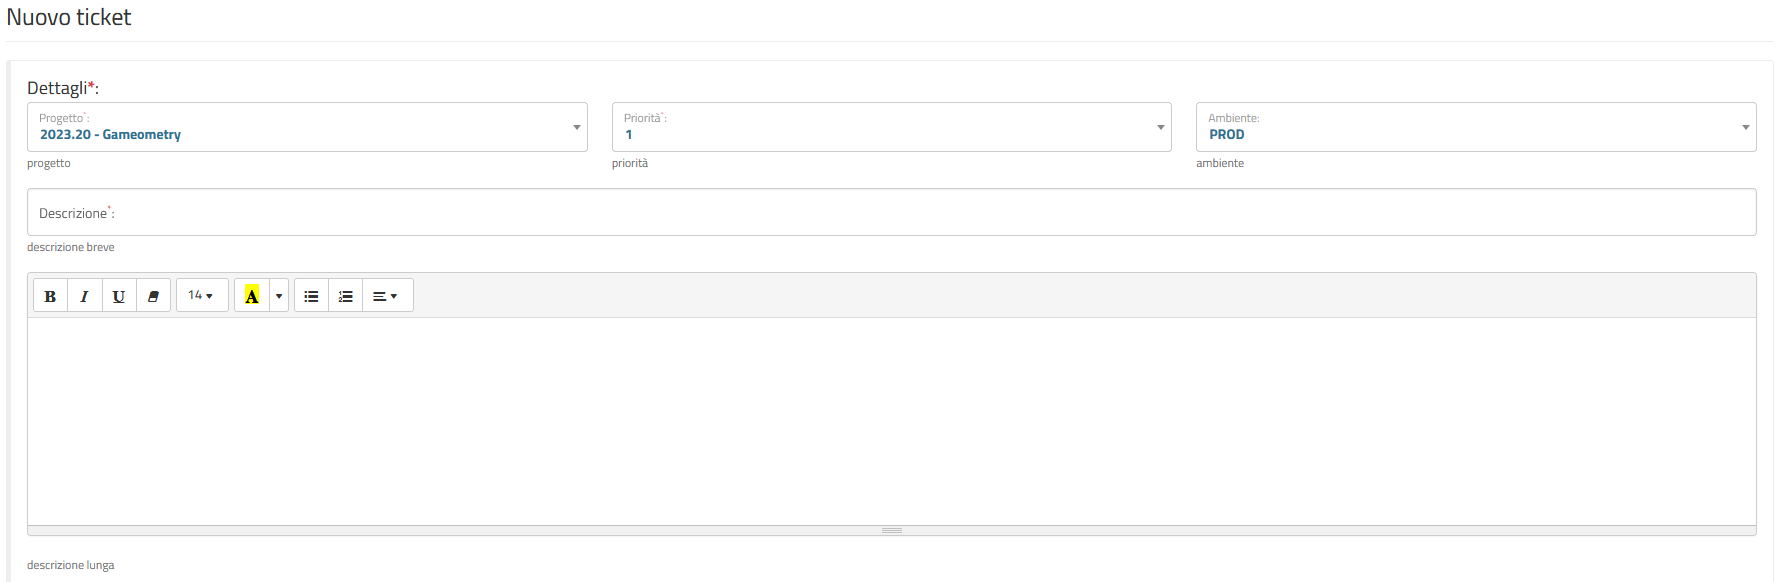
\includegraphics[width=1.5\columnwidth]{newTicket-Step2-prima parte} 
\end{figure}

\begin{figure}[H]
\bigskip
	\centering

        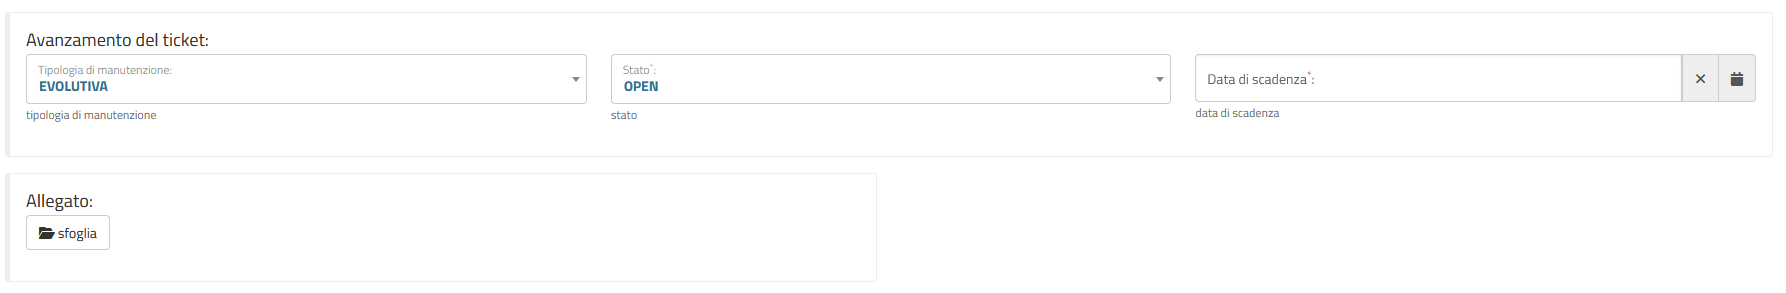
\includegraphics[width=1.5\columnwidth]{newTicket-Step2-seconda parte} 
    \caption{Nuovo Ticket - Step 2}
\end{figure}

\bigskip
\section{Ricerca Ticket}
La pagina di ricerca Ticket offre un spazio in cui vengono visualizzati tutti i ticket secondo i criteri di ricerca. I filtri selezionabili si trovano sul menu a sinistra della pagina e per effettuare la ricerca basta premere sul pulsante "Cerca". Per ogni ticket presente nella lista sono presenti i campi delle caratteristiche che lo rappresentano. Inoltre sono disponibili i pulsanti di modifica e di dettaglio.

\begin{figure}[H]
\bigskip
	\centering
    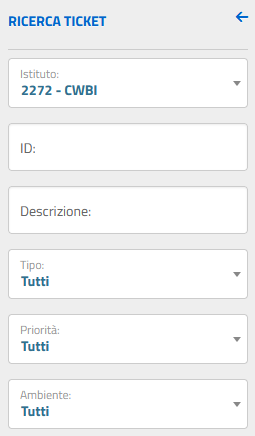
\includegraphics[width=0.35\columnwidth]{ricercaTicket1.1} 
        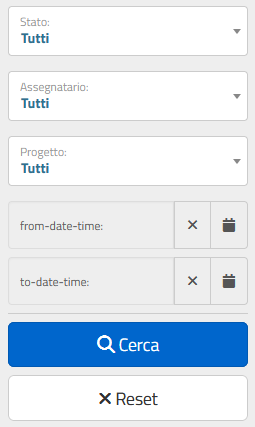
\includegraphics[width=0.35\columnwidth]{ricercaTicket1.2} 
\end{figure}

\begin{figure}[H]
\bigskip
     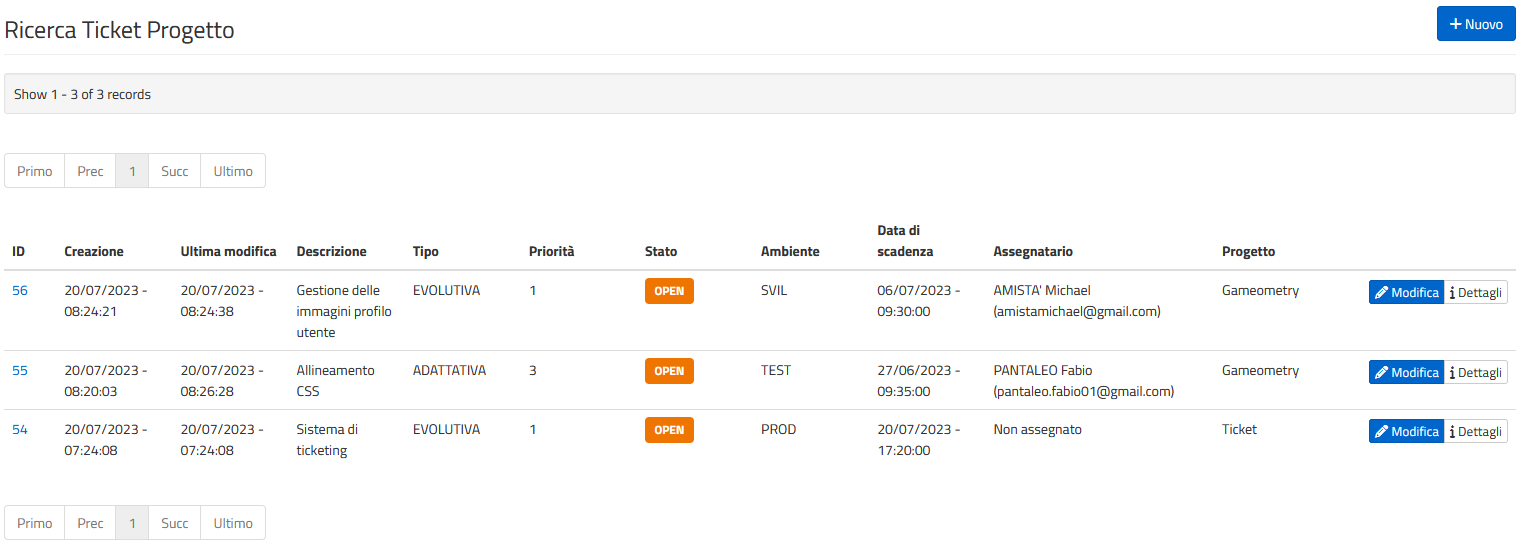
\includegraphics[width=1.3\columnwidth]{ricercaTicket2} 
    \caption{Ricerca Ticket}
\end{figure}

\bigskip
\section{Dettaglio Ticket}
Il dettaglio di un ticket è visualizzato attraverso il pulsante di "Dettaglio" presente in ogni riga delle liste che visualizzano i ticket. La pagina di dettaglio, come dice il nome, visualizza le caratteristiche del ticket in modo dettagliato. \\ 
La parte iniziale della pagina è composta da:\
\medskip
\\textbf{Parte sinistra}
\begin{itemize}
\item \textit{Titolo del Ticket};
\item \textit{Stato};
\item \textit{Priorità};
\item \textit{Tipo};
\item \textit{Ambiente}.
\end{itemize}

\medskip
\noindent
\textbf{Parte destra}
\begin{itemize}
\item \textit{Download dell'allegato};
\item \textit{Chiudi/Apri};
\item \textit{Modifica};
\item \textit{Elimina};
\end{itemize}
\bigskip
\bigskip
\begin{figure}[H]
	\centering
	    
\includegraphics[width=1.1\columnwidth]{dettaglioTicket1} 
     
\includegraphics[width=0.7\columnwidth]{dettaglioTicket2} 
    \caption{Parte iniziale Dettaglio Ticket}
\end{figure}


\noindent
La parte centrale è composta dalle rimanenti caratteristiche del ticket.\\
\bigskip
\begin{figure}[H]
	\centering
    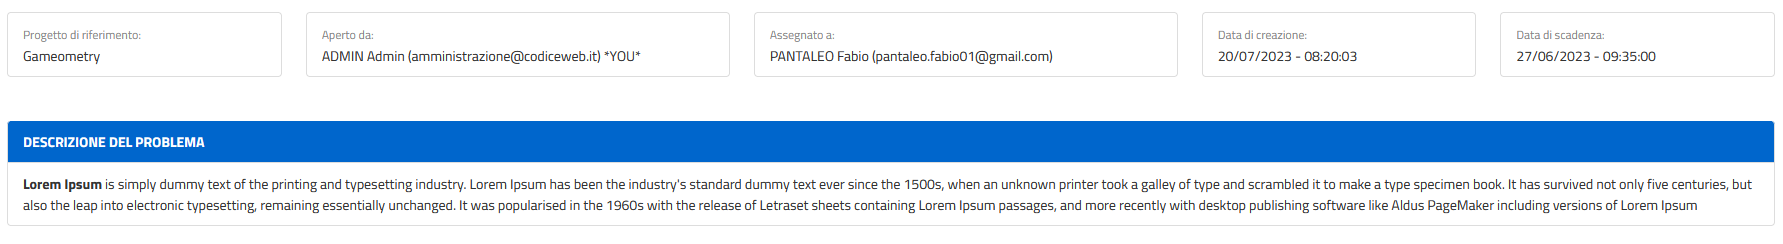
\includegraphics[width=1.25\columnwidth]{dettaglioTicket3} 
\caption{Parte Centrale Dettaglio Ticket}
\end{figure}

\noindent
A fine pagina è posizionata la sezione dei commenti in cui sono presenti tutti i commenti inseriti dagli utenti, con la possibilità di pubblicare un nuovo commento. 

\begin{figure}[H]
	\centering
    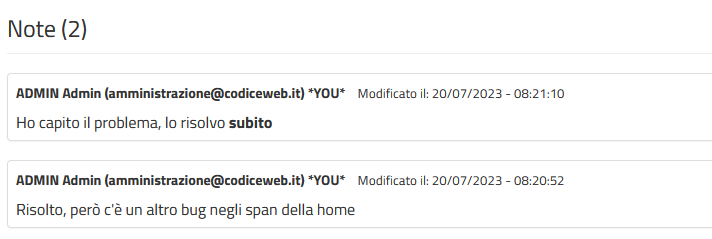
\includegraphics[width=1.2\columnwidth]{dettaglioTicket4} 
\caption{Commenti Dettaglio Ticket}
\end{figure}
\newpage
\section{Commento Ticket}
Questa pagina serve per lasciare una nota per un ticket.


\begin{figure}[H]
	\centering
    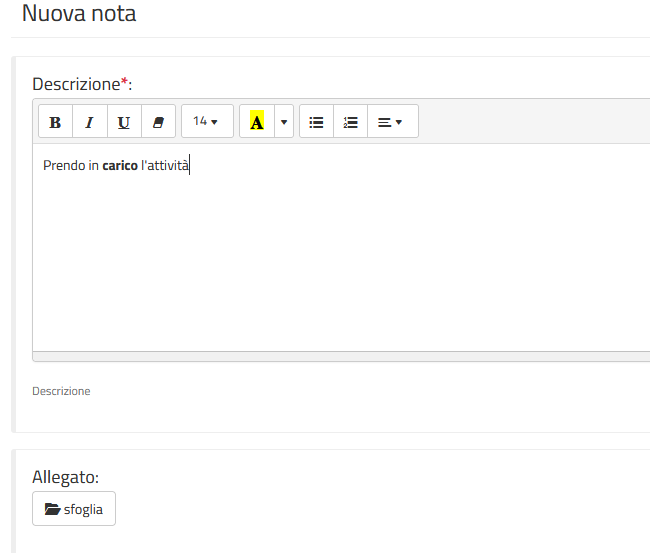
\includegraphics[width=0.8\columnwidth]{nota} 
\caption{Commenti Dettaglio Ticket}
\end{figure}
